\section{METODOLOGÍA SCRUM}

Basándose en \parencite{pressman2010ingenieria}, la \textit{Metodología SCRUM} es un método de desarrollo ágil de software centrado en guiar actividades de desarrollo dentro de un proceso de análisis a través de fases secuenciales estructurales: requerimientos, análisis, diseño, evolución y entrega. La \textit{SCRUM} acentúa el uso de un conjunto de patrones de proceso del software que han demostrado ser eficaces para proyectos con plazos de entrega \textbf{muy apretados}, requerimientos cambiantes y negocios críticos. 

En proyectos relacionados con los \textit{Sistemas de Recomendación} la metodología \textit{SCRUM} es útil por su enfoque iterativo, incremental y adaptativo.

\begin{figure}[h!]
    \centering
    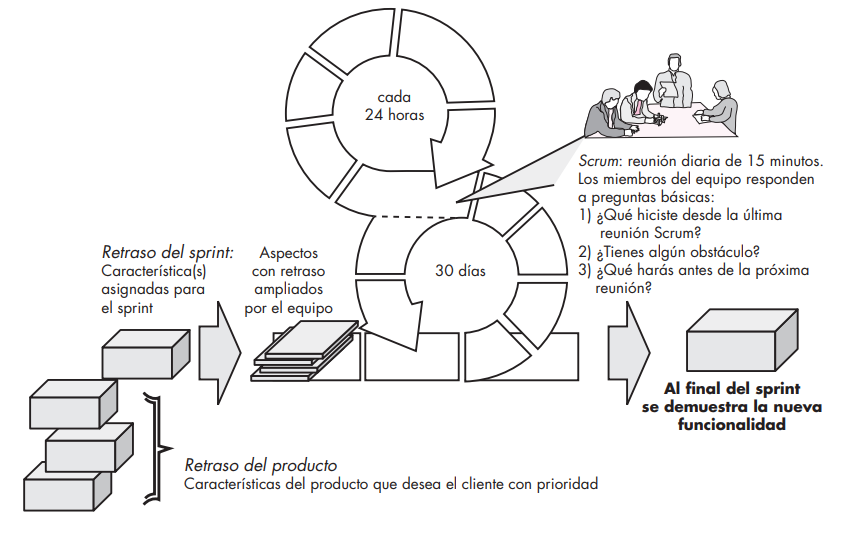
\includegraphics[width=1\linewidth]{SCRUM.png}
    \caption{Descripción del ciclo de vida SCRUM \parencite{pressman2010ingenieria}.}
    \label{fig:SCRUM}
\end{figure}

En la \Cref{fig:SCRUM} se muestra el ciclo de vida de un sistema basado en la metodología \textit{SCRUM}, además, se puede ver que se incorpora un conjunto de patrones del proceso que ponen énfasis en las prioridades del proyecto, las unidades de trabajo agrupadas, la comunicación y la retroalimentación frecuente con el cliente.

Siguiendo a \parencite{pressman2010ingenieria}, algunos de los conceptos más importantes para entender la metodología \textit{SCRUM} son los siguientes: 

\newpage

\begin{definition}
    El \textbf{Retraso} se define como la lista de prioridades de los requerimientos o características del proyecto que dan al cliente un valor del negocio.
\end{definition}

\begin{definition}
    Los \textbf{Sprints} consisten en unidades de trabajo que se necesitan para alcanzar un requerimiento definido en el retraso que debe ajustarse en una caja de tiempo.
\end{definition}

Además de estos conceptos, existen roles, artefactos y ceremonias que describen el proceso de desarrollo mediante la metodología \textit{SCRUM}, basándose en \parencite{sachdeva2016scrum} se definen de manera general los conceptos representado en \Cref{fig:ScrumConceptos}.

\begin{figure}[h!]
    \centering
    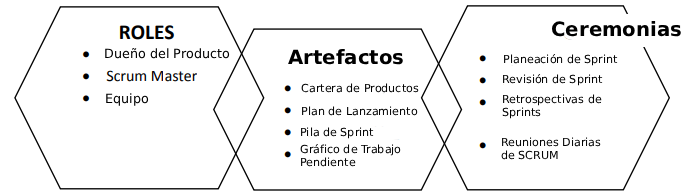
\includegraphics[width=1\linewidth]{ScrumConceptos.png}
    \caption{Conceptos Fundamentales de la Metodología SCRUM \parencite{sachdeva2016scrum}}
    \label{fig:ScrumConceptos}
\end{figure}

\textbf{ROLES}

Una ventaja importante de la Metodología \textit{SCRUM} es que, en comparación con otras metodologías de Ingeniería de Software, no requieren de un lider de proyecto. En compensación, se dividen las responsabilidades en tres roles importantes.

\begin{itemize}
    \item \textbf{Dueño del Producto: } Es el responsable de visión general del producto. Reune y prioriza los requerimientos del producto.
    \item \textbf{Scrum Master: } El Scrum Master es el responsable de que las reglas de la metodología se sigan de manera apropiada, además de tomar control de problemas emergentes.
    \item \textbf{Equipo:} Es un conjunto organizado de personas responsables de la creación y de la calidad del producto. Este equipo debe incluir los roles de testers, diseñadores y \textit{dev ops}.
\end{itemize}

\newpage

\textbf{ARTEFACTOS}

En \textit{SCRUM} los \textbf{artefactos} son los elementos clave de información que se utilizan para asegurar la transparencia, inspección y adaptación en el desarrollo del producto. 

\begin{itemize}
    \item \textbf{Cartera de Productos:} Enlista los requerimientos del producto que deben ser desarrollados. Es la lista principal de todas las funcionalidades deseadas en el producto final.
    \item \textbf{Plan de Lanzamiento: } Plan que describe los objetivos esperados en el lanzamiento, los elementos prioritarios pertenecientes a la cartera de productos y las funcionalidades que el lanzamiento agregará. Además, establece una posible fecha de entrega y el costo esperado.
    \item \textbf{Pila de Sprint: } Consiste de un conjunto de tareas derivadas de la Cartera de Productos segmentando los requerimientos en tareas específicas. Esta pila de sprint esta diseñada para ser modificada únicamente por el equipo de trabajo.
    \item \textbf{Gráfico de Trabajo Pendiente: } Durante un sprint los elementos visuales pueden ser de gran ayuda para el equipo de desarrollo. Este gráfico se centra en la cantidad de trabajo pendiente en la Pila de Sprint y el tiempo estimado restante para la entrega.
\end{itemize}

\textbf{CEREMONIAS}

Las ceremonias son reuniones que buscan dar una estructura clara a cada sprint.

\begin{itemize}
    \item \textbf{Planeación de Sprint: } Esta reunión planea una nueva iteración. En general, se dividen en dos partes: Determinar qué se va a hacer en el siguiente Sprint y cómo será construido el producto.
    \item \textbf{Revisión de Sprint: } Toma lugar al final de un Sprint y tiene como objetivo que el equipo presente las funcionalidades desarrolladas al dueño del producto.
    \item \textbf{Retrospectiva del Sprint: } Se centra en discutir los logros y las áreas de oportunidad durante el proceso de desarrollo.
    \item \textbf{Reunión Diaria de SCRUM: } Esta enfocada en que los integrantes del equipo expliquen en qué han estado trabajando desde la última reunión diaria y lo que planean hacer hasta la siguiente reunión.
\end{itemize}

Según \parencite{pressman2010ingenieria}, una de las características más importantes de \textit{SCRUM} es que supone la existencia del caos. Esta metodología permite que un equipo de software trabaje con éxito en un mundo en el que es imposible eliminar la \textit{incertidumbre}.







